\documentclass[11pt,a4paper]{article}

\usepackage[margin=22mm,headheight=15pt]{geometry}
\usepackage{amsmath}
\usepackage{booktabs}
\usepackage{graphicx}
\usepackage{microtype}
\usepackage{siunitx}
\usepackage{xcolor}
\usepackage{hyperref}
\usepackage{caption}
\usepackage{subcaption}
\usepackage{fancyhdr}
\usepackage{enumitem}
\usepackage{array}
\usepackage{tabularx}
\usepackage{placeins}
\usepackage[T1]{fontenc}
\usepackage{helvet}
\renewcommand{\familydefault}{\sfdefault}

\definecolor{cmsblue}{HTML}{155A8A}
\definecolor{darkblue}{HTML}{103B5C}
\definecolor{softgray}{HTML}{F2F4F5}
\hypersetup{colorlinks=true,linkcolor=cmsblue,urlcolor=cmsblue,citecolor=cmsblue}
\captionsetup{font=small,labelfont=bf,labelsep=period}
\sisetup{separate-uncertainty=true,round-mode=places,round-precision=4}

\pagestyle{fancy}
\fancyhf{}
\lhead{CMS Run-3 all-hadronic stop analysis}
\rhead{Low-$p_{\mathrm{T}}$ lepton ID scale factors}
\cfoot{\thepage}
\renewcommand{\headrulewidth}{0.4pt}

\newcommand{\pt}{p_{\mathrm{T}}}
\newcommand{\abseta}{|\eta|}
\newcommand{\eff}{\varepsilon}
\newcommand{\SF}{\mathrm{SF}}
\newcommand{\NA}{--}

\title{\vspace{-12mm}\color{darkblue}\textbf{Measurement of Low-$p_{\mathrm{T}}$ Electron and Muon Identification Scale Factors in 2024 Data}\\[3mm]
\large CMS Run-3 all-hadronic stop analysis}
\author{Internal physics report}
\date{4 August 2026}

\begin{document}
\maketitle

\begin{abstract}
The all-hadronic stop search vetoes electrons and muons down to transverse momenta below the lower boundary of the standard lepton scale-factor inputs used in the analysis.  Dedicated data-to-simulation identification scale factors are therefore measured for veto electrons and loose muons in the interval $5<\pt<10\,\mathrm{GeV}$.  The measurement uses the $J/\psi\to\ell\ell$ resonance in 2024 ParkingSingleMuon data and double-$J/\psi$ simulation.  Trigger bias is controlled by making the parking-muon requirement independent of the electron pair and, for the muon channel, by requiring a third reference muon distinct from the measured pair.  Pass and fail invariant-mass spectra are fit simultaneously in data and simulation.  This report defines the physics samples, tag-and-probe selections, fit model, uncertainty construction, measured scale factors, and the statistical limitations of the present determination.  In the forward-electron interval, where the failing-probe peak does not satisfy the adopted significance requirement, the correction candidate uses a unity central value with a measurement-derived uncertainty.  The results are labeled by the data-taking year rather than by an integrated luminosity because a trigger-specific luminosity determination is not part of this measurement.  Independent validation by the relevant CMS Physics Object Groups (POGs) is needed in future work.
\end{abstract}

\section{Physics motivation and scope}

The lost-lepton control region (LLCR) and lepton-vetoed signal selections depend on the probability for a reconstructed low-$\pt$ lepton to satisfy the analysis identification requirement.  In the previous implementation, objects below $10\,\mathrm{GeV}$ were evaluated at the boundary of the standard correction.  Such clipping replaces the unknown low-$\pt$ response by the response at $10\,\mathrm{GeV}$ and removes any genuine dependence on detector region or momentum.  The present measurement directly covers the missing interval.

The measured quantities are deliberately \emph{ID only}:
\begin{itemize}[leftmargin=6mm,itemsep=1mm]
  \item the electron numerator is the analysis veto identification, \texttt{cutBased}$\geq1$;
  \item the muon numerator is \texttt{looseId};
  \item probe mini-isolation is not included in either pass/fail definition.
\end{itemize}
This factorization prevents an ID correction from absorbing a separate isolation efficiency.  The scale factor is a correction to simulated event weights and does not alter the object selection in data.

\section{Data, simulation, and reference-trigger strategy}

\subsection{Data sample}

Both channels use the 2024 \path{ParkingSingleMuon} primary datasets in the MINIv6NANOv15 NanoAOD processing.  Events are restricted to certified 2024 luminosity sections with \path{Cert_Collisions2024_378981_386951_Golden.json} and pass the standard Run-3 event-cleaning filters.  The reference decision is the logical OR
\begin{equation}
  \mathrm{HLT\_Mu9\_Barrel\_L1HP10\_IP6}
  \;\lor\;
  \mathrm{HLT\_Mu10\_Barrel\_L1HP11\_IP6}.
\end{equation}
The plots carry the label ``2024 (13.6 TeV).''  No numerical integrated luminosity is quoted because the effective luminosity of this displaced-muon parking selection has not been evaluated in this work.

\subsection{Simulation samples}

The electron channel uses
\begin{center}
\small\path{/SPS-JpsiJpsiToMuMuEE_TuneCP5_13p6TeV_pythia8/RunIII2024Summer24NanoAODv15-150X_mcRun3_2024_realistic_v2-v2/NANOAODSIM}.
\end{center}
One $J/\psi$ supplies the muon-trigger side of the event while the second supplies the $J/\psi\to ee$ tag-and-probe pair.

The muon channel uses
\begin{center}
\small\path{/SPS-JpsiJpsiTo4Mu_Fil-4Mu_TuneCP5_13p6TeV_pythia8/RunIII2024Summer24NanoAODv15-150X_mcRun3_2024_realistic_v2-v4/NANOAODSIM}.
\end{center}
The four-muon final state permits a disjoint reference muon and a measured $J/\psi\to\mu\mu$ pair in the same event.  Simulated events are weighted by the generator weight and the 2024 pileup correction \texttt{Collisions24\_BCDEFGHI\_goldenJSON}.  The parking HLT requirement is applied to data only; the same offline reference topology is imposed on simulation.

\subsection{Avoiding trigger bias}

For electrons, the parking-muon trigger is external to the measured $ee$ pair.  Neither the electron tag nor probe is required to match a trigger object or an electron HLT path.  The electron efficiency therefore probes the offline electron requirement rather than a convolution with an electron trigger.

For muons, either measured leg could otherwise be responsible for the parking decision.  A third tight muon is consequently required with $\pt>12\,\mathrm{GeV}$ and $\abseta<1.5$.  This reference muon must be distinct from both tag-and-probe legs.  Neither measured leg is trigger matched or required to pass isolation.  The same disjoint three-muon topology is imposed on the four-muon simulation.

\section{Tag-and-probe definitions}

Opposite-charge, distinct tag-probe pairs are formed and their invariant mass is computed from the reconstructed four-vectors.  A probe enters either the passing or failing spectrum, never both.

\begin{table}[htbp]
\centering
\caption{Offline definitions used in the two ID-only measurements.}
\begin{tabularx}{\textwidth}{>{\bfseries}p{24mm}XX}
\toprule
 & Electron channel & Muon channel \\
\midrule
Tag & Tight electron, $\pt>5\,\mathrm{GeV}$, $\mathrm{miniPFRelIso\_all}<0.1$; no HLT match & Tight muon, $\pt>5\,\mathrm{GeV}$; no isolation or HLT match \\
Probe denominator & Reconstructed GSF electron, $5<\pt<10\,\mathrm{GeV}$, ECAL fiducial, conversion veto, lost hits $\leq1$; no cut-based ID or isolation requirement & Tracker muon, $5<\pt<10\,\mathrm{GeV}$, $\abseta<2.4$; no LooseID or isolation requirement \\
Passing probe & \texttt{cutBased}$\geq1$ & \texttt{looseId} \\
Failing probe & Denominator probe not satisfying \texttt{cutBased}$\geq1$ & Denominator probe not satisfying \texttt{looseId} \\
Reference topology & Parking-muon trigger external to the $ee$ pair & A third tight barrel muon distinct from the $\mu\mu$ pair \\
\bottomrule
\end{tabularx}
\end{table}

The electron ECAL transition region is excluded before histogram filling.  Thus the histogram interval labeled $1.44<\abseta<2.5$ physically contains probes with $1.566<\abseta<2.5$.

\section{Efficiency and scale-factor extraction}

For each probe bin, passing and failing mass spectra are described by
\begin{align}
  M_{\mathrm{pass}}(m) &= N_{\mathrm{sig}}\,\eff\,S_{\mathrm{pass}}(m)
  + N_{\mathrm{bkg,pass}} B_{\mathrm{pass}}(m),\\
  M_{\mathrm{fail}}(m) &= N_{\mathrm{sig}}(1-\eff)S_{\mathrm{fail}}(m)
  + N_{\mathrm{bkg,fail}} B_{\mathrm{fail}}(m).
\end{align}
The efficiency $\eff$ is a parameter of the simultaneous pass/fail fit, equivalent to
\begin{equation}
  \eff = \frac{N_{\mathrm{sig}}^{\mathrm{pass}}}
  {N_{\mathrm{sig}}^{\mathrm{pass}}+N_{\mathrm{sig}}^{\mathrm{fail}}}.
\end{equation}
Data and simulation are fit independently, and the correction is
\begin{equation}
  \SF(\pt,\abseta)=\frac{\eff_{\mathrm{data}}(\pt,\abseta)}
  {\eff_{\mathrm{MC}}(\pt,\abseta)}.
\end{equation}
The scale factor is therefore determined by the fitted resonant signal yields after subtraction of the nonresonant component.  It is not determined by the raw pass fraction or by the peak height in a single mass bin.

\subsection{Nominal line shape and background}

The nominal signal model is a double-sided Crystal Ball (DSCB) function.  The Gaussian core represents detector resolution around the $J/\psi$ pole, while independent power-law tails accommodate radiative and reconstruction effects.  The nominal fit shares the signal response between passing and failing probes; an independent pass/fail response is included as a model variation.

The electron spectra are fit over $2.0<m_{ee}<4.0\,\mathrm{GeV}$ with a Chebyshev background.  The muon spectra are fit over $2.6<m_{\mu\mu}<3.6\,\mathrm{GeV}$ with an exponential nominal background.  The nominal displayed bin width is $40\,\mathrm{MeV}$.  The red curve in the figures is the continuous signal-plus-background model, and the blue curve is its background component.

\subsection{Probe binning}

The electron result retains two momentum bins, $5$--$7$ and $7$--$10\,\mathrm{GeV}$, and three detector regions: $0<\abseta<0.8$, $0.8<\abseta<1.44$, and $1.566<\abseta<2.5$.  The muon study was initially evaluated on a 1-GeV momentum grid.  The final candidate combines $5<\pt<10\,\mathrm{GeV}$ and uses $0<\abseta<0.9$, $0.9<\abseta<1.2$, and $1.2<\abseta<2.4$.  This combination increases the statistical sensitivity of the failing-probe resonance while retaining the principal detector regions.

\section{Uncertainty model}

The statistical uncertainty is propagated from the fitted data and simulation efficiencies,
\begin{equation}
  \sigma_{\mathrm{stat}}(\SF)=\SF
  \sqrt{\left(\frac{\sigma_{\eff,\mathrm{data}}}{\eff_{\mathrm{data}}}\right)^2
  +\left(\frac{\sigma_{\eff,\mathrm{MC}}}{\eff_{\mathrm{MC}}}\right)^2}.
\end{equation}
Fit-model stability is evaluated with five alternatives to the nominal determination:
\begin{enumerate}[leftmargin=7mm,itemsep=1mm]
  \item a Gaussian-exponential signal in place of the DSCB;
  \item the alternate background family (exponential or Chebyshev);
  \item independent passing and failing signal responses;
  \item a narrower mass window;
  \item a $20\,\mathrm{MeV}$ mass binning in place of $40\,\mathrm{MeV}$.
\end{enumerate}
The fit systematic is the largest absolute scale-factor displacement among these alternatives.  The pileup systematic is the largest displacement obtained with the up/down pileup weights.  They are combined as
\begin{align}
  \sigma_{\mathrm{syst}}^2 &= \sigma_{\mathrm{fit}}^2+\sigma_{\mathrm{PU}}^2,\\
  \sigma_{\mathrm{total}}^2 &= \sigma_{\mathrm{stat}}^2+\sigma_{\mathrm{syst}}^2.
\end{align}

A fit is retained only when the nominal and all model variations converge for both data and simulation and the failing-probe component is statistically identifiable.  The latter is quantified by
\begin{equation}
  Z_{\mathrm{fail}}=\frac{1-\eff}{\sigma_{\eff}}\geq3.
\end{equation}

\section{Electron ID-only result}

\begin{figure}[htbp]
\centering
\begin{subfigure}{0.49\textwidth}
  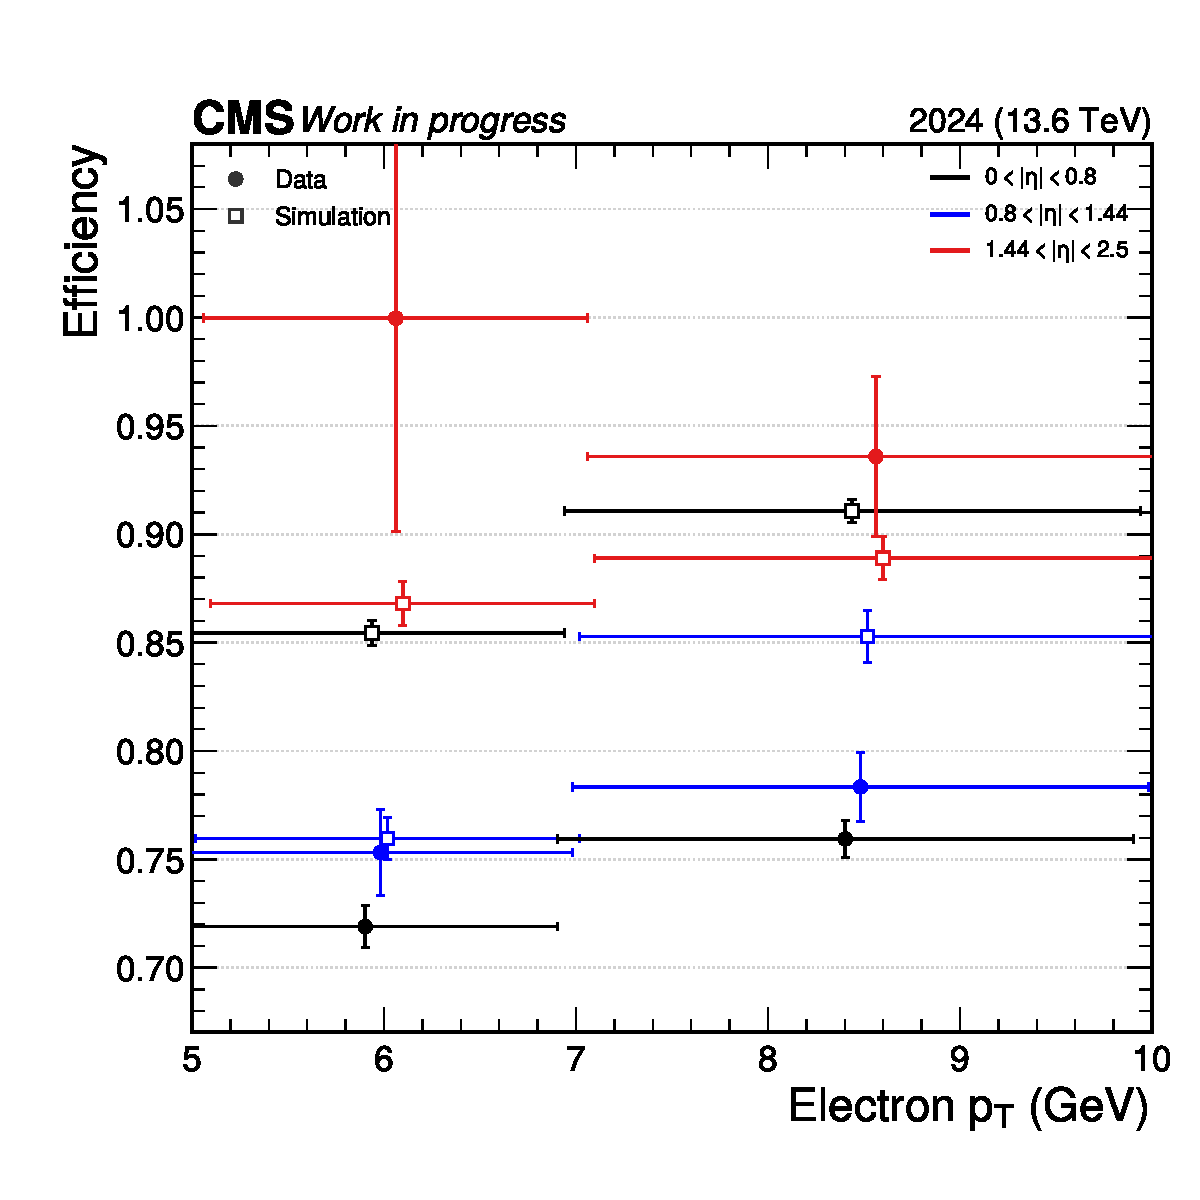
\includegraphics[width=\textwidth]{electron/efficiency.pdf}
  \caption{Efficiencies in data and simulation.}
\end{subfigure}\hfill
\begin{subfigure}{0.49\textwidth}
  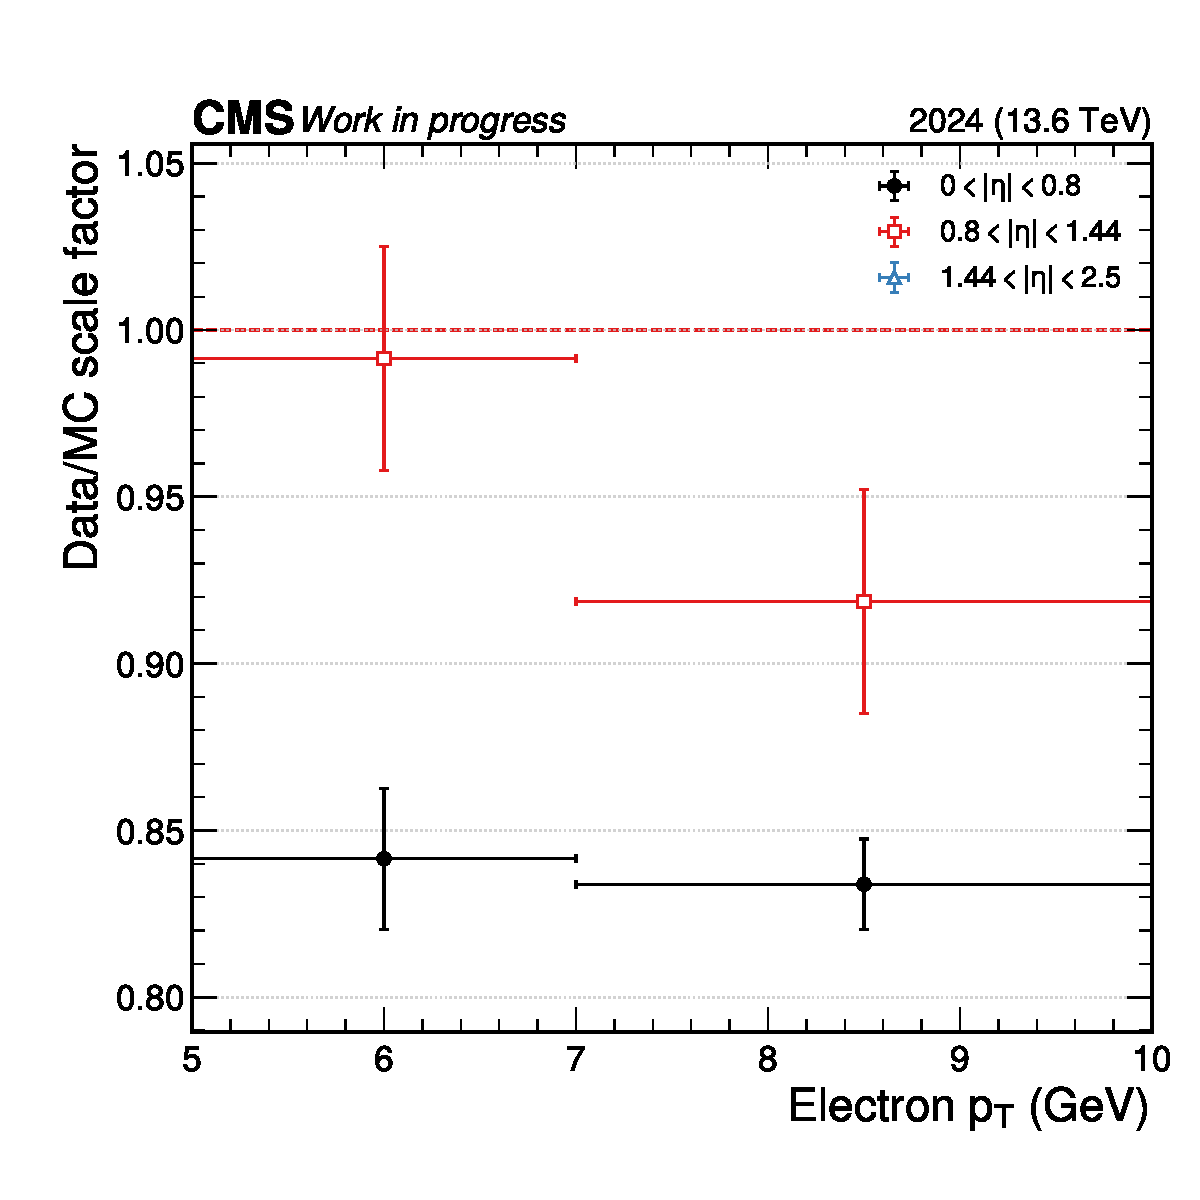
\includegraphics[width=\textwidth]{electron/scale_factor.pdf}
  \caption{Data-to-simulation scale factors.}
\end{subfigure}
\caption{Veto-electron ID-only measurement.  The combined efficiency figure uses color for the detector region, filled circles for data, and open squares for simulation.}
\end{figure}

\begin{table}[htbp]
\centering
\caption{Electron efficiencies, scale factors, and uncertainties.  The forward rows report the fitted efficiencies and failing-probe significance.  Their correction-candidate central values are set to unity; the quoted total uncertainty is the quadrature sum of the fitted Data/MC ratio's displacement from unity and its propagated statistical uncertainty.}
\resizebox{\textwidth}{!}{%
\begin{tabular}{cccccccccc}
\toprule
$\abseta$ & $\pt$ [GeV] & $\eff_{\mathrm{data}}$ & $\eff_{\mathrm{MC}}$ & $\SF$ & stat. & fit & PU & total & $Z_{\mathrm{fail}}$ \\
\midrule
0--0.8 & 5--7 & 0.7190 & 0.8544 & 0.8415 & 0.0127 & 0.0166 & 0.0032 & 0.0211 & 28.82 \\
0--0.8 & 7--10 & 0.7594 & 0.9107 & 0.8339 & 0.0104 & 0.0044 & 0.0075 & 0.0136 & 28.76 \\
0.8--1.44 & 5--7 & 0.7532 & 0.7596 & 0.9915 & 0.0288 & 0.0121 & 0.0122 & 0.0335 & 12.54 \\
0.8--1.44 & 7--10 & 0.7835 & 0.8529 & 0.9186 & 0.0226 & 0.0218 & 0.0115 & 0.0335 & 13.65 \\
1.566--2.5 & 5--7 & 0.9997 & 0.8680 & 1.0000 & \NA & \NA & \NA & 0.1900 & 0.003 \\
1.566--2.5 & 7--10 & 0.9358 & 0.8889 & 1.0000 & \NA & \NA & \NA & 0.0683 & 1.73 \\
\bottomrule
\end{tabular}}
\end{table}

In the two barrel regions, the measured veto-electron efficiency is substantially lower in data than in simulation for three of the four bins, producing scale factors below unity.  The $0.8<\abseta<1.44$, $5<\pt<7\,\mathrm{GeV}$ bin is compatible with unity within its total uncertainty.  In the forward region the fitted failing-probe peak has limited statistical significance, most strongly in the $5$--$7\,\mathrm{GeV}$ bin.  The correction candidate therefore returns a nominal value of one in both forward bins.  A nonzero symmetric uncertainty is retained: if $r=\eff_{\mathrm{data}}/\eff_{\mathrm{MC}}$ and $\sigma_r$ is its propagated statistical uncertainty, the adopted width is $\sqrt{(r-1)^2+\sigma_r^2}$.  This gives $19.0\%$ and $6.83\%$ in the $5$--$7$ and $7$--$10\,\mathrm{GeV}$ bins, respectively.  The corresponding $Z_{\mathrm{fail}}$ values document the present statistical sensitivity.  Future independent validation by the relevant electron POG is needed.

\begin{figure}[htbp]
\centering
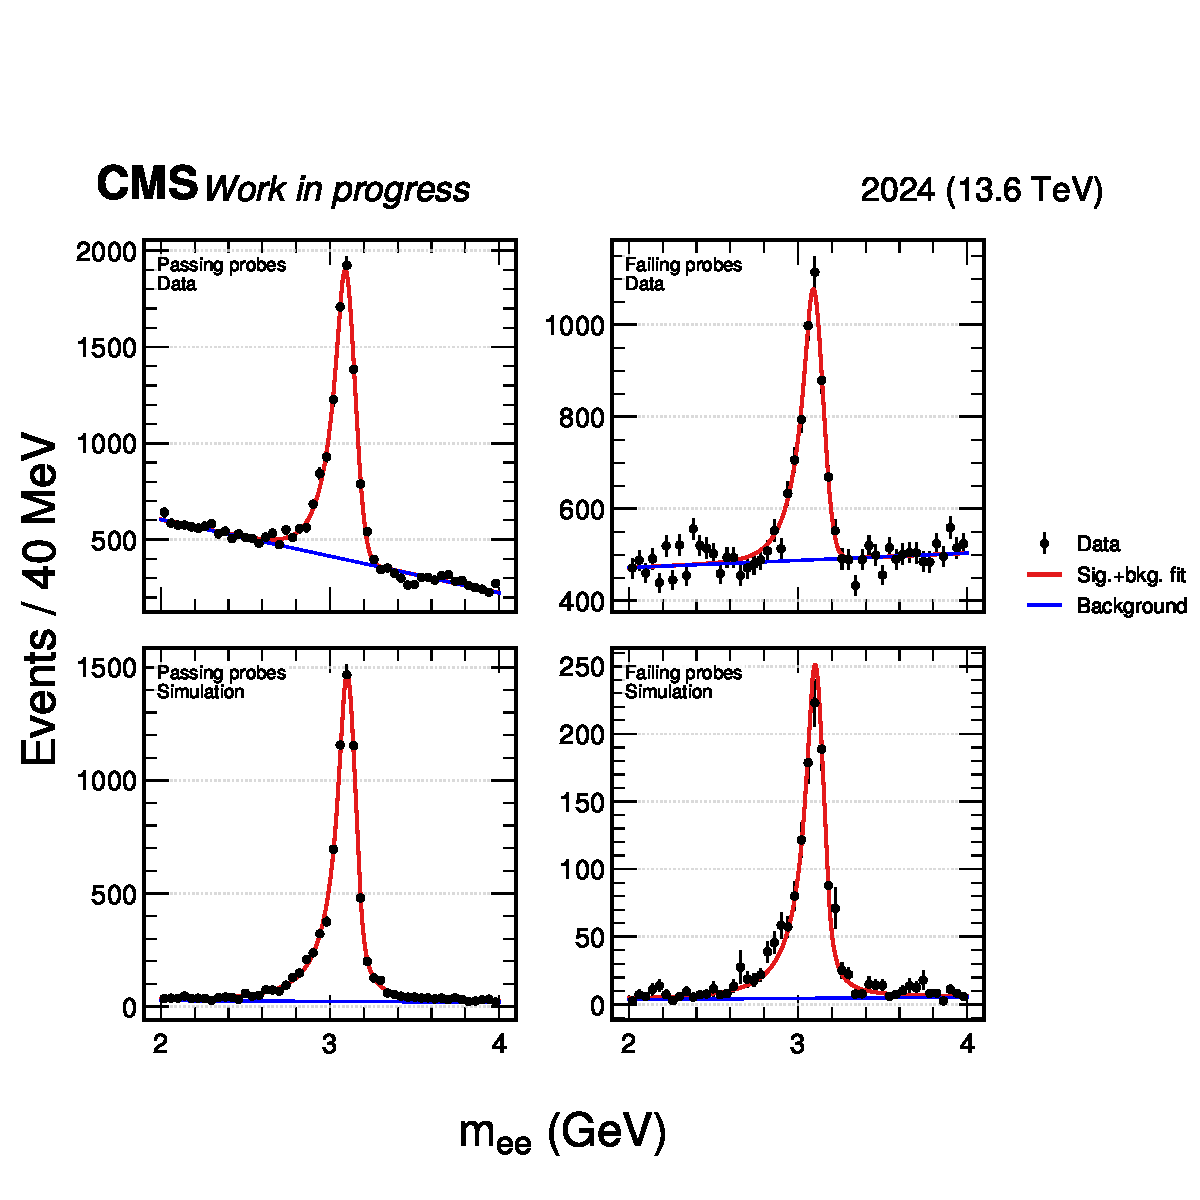
\includegraphics[width=0.76\textwidth]{electron/mass_fit_bin_00.pdf}
\caption{Electron pass/fail mass fit for $0<\abseta<0.8$ and $5<\pt<7\,\mathrm{GeV}$.  The four panels show data passing, data failing, simulation passing, and simulation failing probes.}
\end{figure}

\begin{figure}[htbp]
\centering
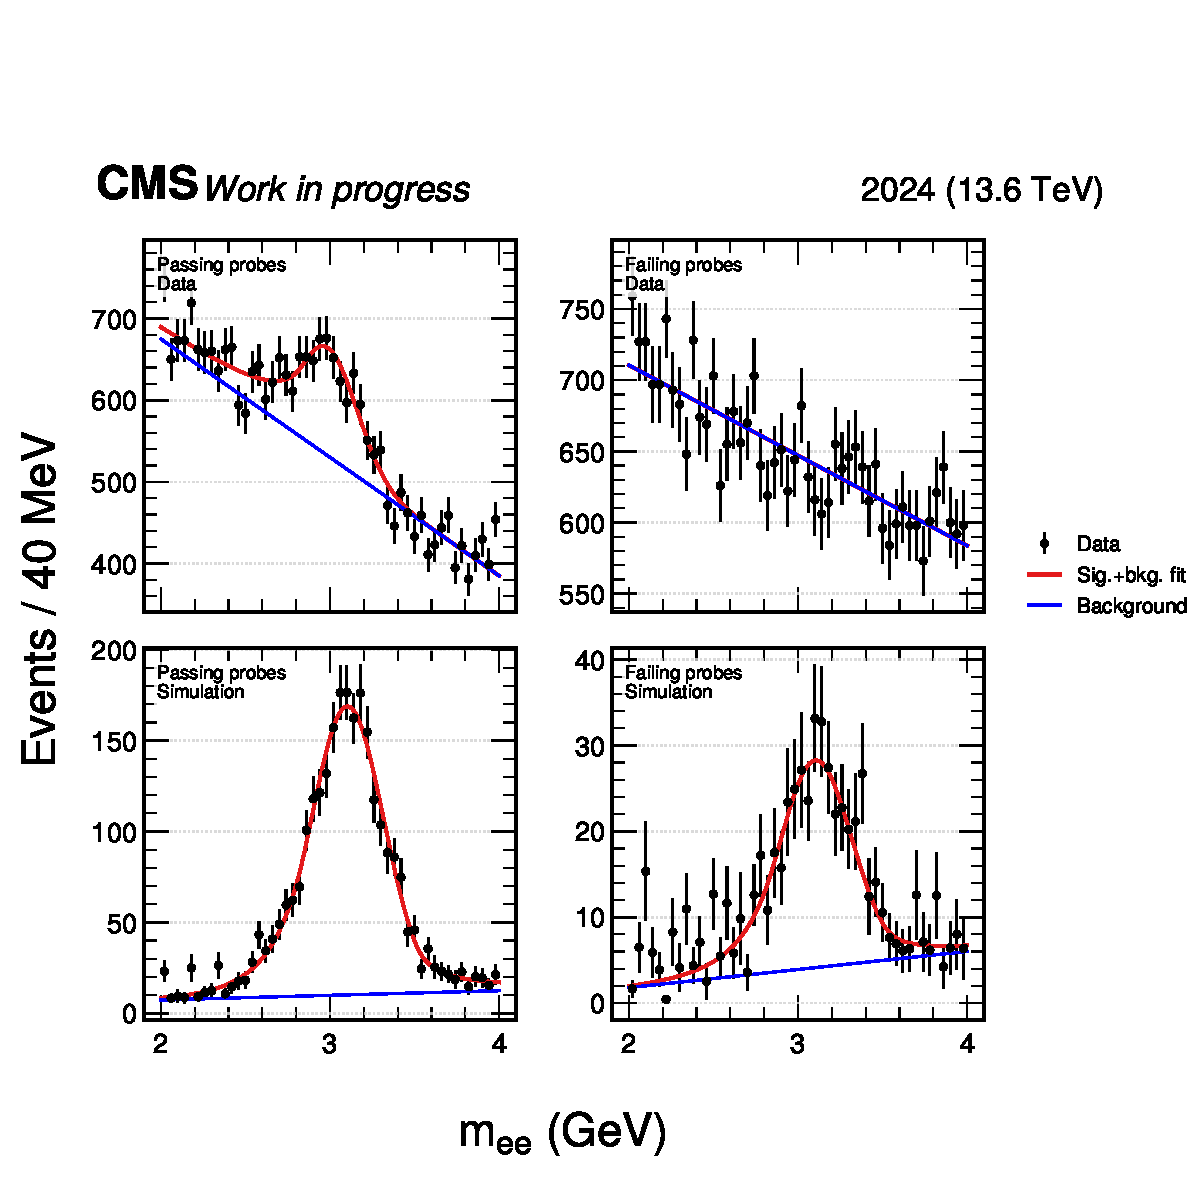
\includegraphics[width=0.76\textwidth]{electron/mass_fit_bin_04.pdf}
\caption{Electron pass/fail mass fit in the forward $5$--$7\,\mathrm{GeV}$ bin.  The weakly identified failing-probe resonance motivates the explicit significance requirement in the fit validation.}
\end{figure}
\FloatBarrier

\section{Muon ID-only result}

\begin{figure}[htbp]
\centering
\begin{subfigure}{0.49\textwidth}
  
\includegraphics[width=\textwidth]{muon/efficiency.pdf}
  \caption{Efficiencies in data and simulation.}
\end{subfigure}\hfill
\begin{subfigure}{0.49\textwidth}
  
\includegraphics[width=\textwidth]{muon/scale_factor.pdf}
  \caption{Data-to-simulation scale factors.}
\end{subfigure}
\caption{Loose-muon ID-only measurement integrated over $5<\pt<10\,\mathrm{GeV}$.}
\end{figure}

\begin{table}[htbp]
\centering
\caption{Muon efficiencies, scale factors, and uncertainties.}
\begin{tabular}{ccccccccc}
\toprule
$\abseta$ & $\eff_{\mathrm{data}}$ & $\eff_{\mathrm{MC}}$ & $\SF$ & stat. & fit & PU & total & $Z_{\mathrm{fail}}$ \\
\midrule
0--0.9 & 0.9849 & 0.9865 & 0.9984 & 0.0011 & 0.0005 & 0.0002 & 0.0012 & 13.98 \\
0.9--1.2 & 0.9844 & 0.9841 & 1.0003 & 0.0018 & 0.0006 & 0.0000 & 0.0019 & 9.50 \\
1.2--2.4 & 0.9921 & 0.9939 & 0.9982 & 0.0014 & 0.0009 & 0.0002 & 0.0017 & 5.76 \\
\bottomrule
\end{tabular}
\end{table}

The loose-muon ID efficiency exceeds $98\%$ in all three detector regions.  The data-to-simulation ratios are within approximately $0.2\%$ of unity, and the total uncertainties range from $0.12\%$ to $0.19\%$.  All three failing-probe peaks exceed the adopted $3\sigma$ identification threshold.  The nominal goodness-of-fit values are larger than unity in several data or simulation spectra, so the alternate line-shape and background variations remain an essential part of the uncertainty.  Future independent validation by the relevant muon POG is needed.

\begin{figure}[htbp]
\centering

\includegraphics[width=0.76\textwidth]{muon/mass_fit_bin_00.pdf}
\caption{Muon pass/fail mass fit for $0<\abseta<0.9$ and $5<\pt<10\,\mathrm{GeV}$.}
\end{figure}
\FloatBarrier

\section{Interpretation for the all-hadronic stop analysis}

The corrections address the exact low-$\pt$ ID definitions entering lepton vetoes and the LLCR.  For an eligible simulated lepton, the nominal scale factor multiplies the event weight and the up/down values define the associated systematic variation.  Above $10\,\mathrm{GeV}$ the standard electron and muon corrections retain their usual role; the present measurement supplies the previously clipped $5$--$10\,\mathrm{GeV}$ interval.  In the highest electron $\abseta$ interval the candidate evaluates to unity nominally and propagates the $19.0\%$ or $6.83\%$ uncertainty according to the electron $\pt$ bin.  Because isolation is excluded from the measured numerator, any isolation scale factor remains a separate multiplicative correction where the analysis definition requires it.

The electron result exhibits a sizeable low-$\pt$ data-to-simulation difference in the central detector, while the muon result is close to unity.  These qualitatively different outcomes are physically plausible: low-energy electron shower reconstruction and cut-based observables are more sensitive to material and detector response than tracker-muon reconstruction and LooseID.  The forward-electron failing sample is statistically limited and is explicitly visible in the accompanying mass fits.  Future comparison with POG reference methods and prescriptions is needed to establish the treatment of this region.

\section{Summary}

Dedicated $J/\psi$ tag-and-probe measurements have been constructed for veto-electron and loose-muon ID efficiencies in 2024 data over $5<\pt<10\,\mathrm{GeV}$.  The parking trigger is external to the measured electron pair, and a disjoint third-muon topology protects the muon measurement from trigger bias.  A simultaneous DSCB-based pass/fail fit isolates the resonant signal from the background and determines the data and simulation efficiencies.  Model, mass-window, binning, response-factorization, and pileup variations are propagated to the total uncertainty.  Four central-electron bins and all three final muon bins satisfy the current fit criteria.  The two forward-electron candidate bins use nominal unity with measurement-derived uncertainties of $19.0\%$ and $6.83\%$, while their mass spectra retain the evidence for the limited failing-probe sensitivity.  Future independent validation by the relevant CMS electron and muon POGs is needed.

\section*{Reference}
\begin{enumerate}[leftmargin=7mm]
  \item CMS Collaboration, CMS-DP-2023/081, low-$\pt$ electron identification efficiency studies using $J/\psi$ tag-and-probe in Run 2.
\end{enumerate}

\end{document}
